\documentclass[10pt]{article}\usepackage[margin=.55in]{geometry}\usepackage[T1]{fontenc}\usepackage{graphicx}\setlength{\parindent}{0pt}\setlength{\parskip}{4pt}\sloppy\begin{document}{\large Independent review: solve4 pivot normalization}\par The nine normalization declarations are faithful to the stated single-row value contract. Fresh checks accepted the seven producer controls and three reviewer controls; a separate readback audited all 19 named declarations. The wrong-unit false theorem was rejected. This review concerns published producer 8659a98a2b9513dc3dcd8300cca4304c582d4cb2.\par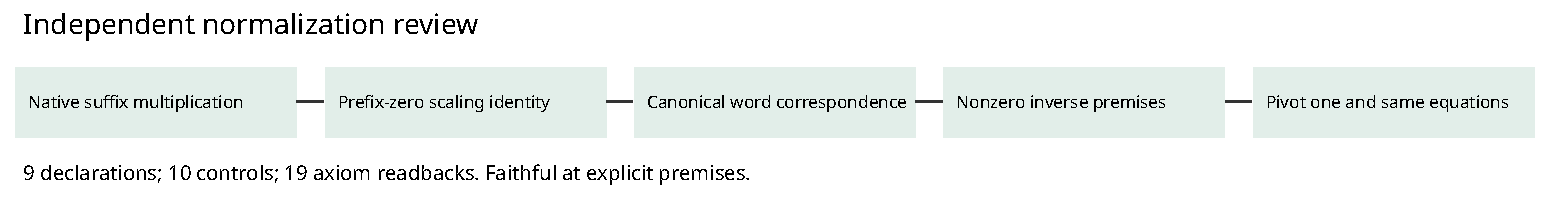
\includegraphics[width=.96\linewidth]{diagram.pdf}\par Source fidelity. The native code finds and swaps a nonzero pivot, computes unit once and scales columns col through 4, including the RHS. The proof models that suffix multiplication expression. Earlier zero coefficients make it equal full-row scaling. Field distributivity gives the residual scaling identity; a nonzero inverse gives equation equivalence and pivot one. The word contract derives canonical output, preserved prefix, pivot one and equivalence for every vector from canonical arithmetic and prime p at most 2\textasciicircum{}32. No output equation is used as a premise.

Explicit obligations. The supplied unit must be canonical and decode to the actual field inverse. The pivot is assumed nonzero in the field and its prefix is assumed zero. These premises are sufficient but native pow/inv, pivot selection, swap, prior-column induction, in-place array semantics and final return still need their own bridge. The producer report states these limits accurately. All three pinned Rust source hashes matched.

Reviewer controls. New exact examples cover column 0 updating the full row, final pivot column 3 updating the RHS, and characteristic 2 word normalization. Existing controls cover a valid inverse instance, equation preservation, zero pivot, wrong unit, zero unit losing equation equivalence and missing-prefix failure. The test-only false theorem rejected by decide remains a separate negative artifact.

Verification and independence. Five fresh Lean calls completed in 21.115096 seconds inside one 300-second wrapper bound. All 28,805 recursive dependency/toolchain hashes were unchanged. Only propext, Classical.choice and Quot.sound appear in the named readbacks. The reviewer authored the prior suffix component but not this normalization proof; context was disclosed before source access, so mutual blindness is not claimed. The prior component's independent verdict remains its separate review. Imported compiled dependencies retain Lean's binary trust boundary; no independent kernel/binary rechecker was run.

Next mathematical bridge. Establish native modular exponentiation/inversion correctness and derive the pivot-prefix and nonzero conditions from selection, swaps and prior columns. No scientific cohort, native solver trajectory or runtime qualification was executed in this review.
\end{document}